\documentclass[border=10pt]{standalone}
\usepackage[utf8]{inputenc}
\usepackage{tikz}
\usetikzlibrary{arrows,decorations.pathmorphing,backgrounds,fit,positioning,shapes.symbols,chains,shapes.geometric,shapes.arrows,calc}

\begin{document}
  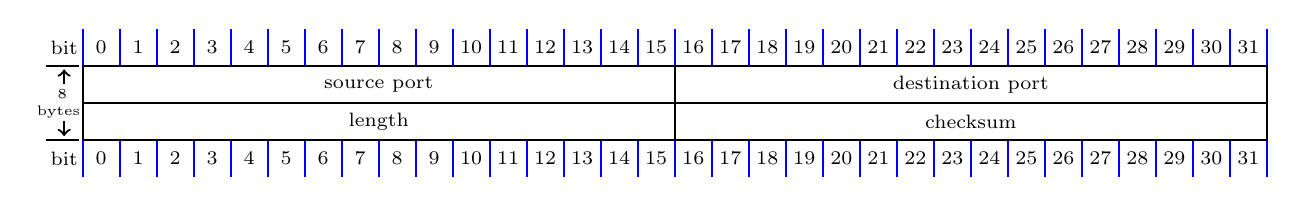
\begin{tikzpicture}[scale=0.47]
	\foreach \x in {0,...,31}
		\node at (\x+0.5,20.5) {\scriptsize \x};
	\foreach \x in {0,...,31}
		\node at (\x+0.5,17.5) {\scriptsize \x};
	\foreach \x in {0,...,32} 
		\draw[thick, blue] (\x,17) -- (\x,21);
	\node[thick] (bit1) at (-0.5,20.5) {\scriptsize bit};
	\node[thick] (bit2) at (-0.5,17.5) {\scriptsize bit};
	\draw [<->, thick] (-0.5, 19.9) -- (-0.5,18.1);
	\draw [thick] (-1, 20) -- (-0.1,20);
	\draw [thick] (-1, 18) -- (-0.1,18);
	\fill[white] (-0.8,19.5) rectangle (-0.1,18.5);
	\node at (-0.55,19.25) {\tiny 8};
	\node at (-0.65,18.75) {\tiny bytes};
	\filldraw[thick,draw=black, fill=white] (0,20) rectangle (16,19); \node (mode) at (8,19.5) {\scriptsize source port};
	\draw[thick, draw=black, fill=white] (16,20) rectangle (32,19); \node (li) at (24,19.5) {\scriptsize destination port};
	\filldraw[thick,draw=black, fill=white] (0,19) rectangle (16,18); \node (mode) at (8,18.5) {\scriptsize length};
	\draw[thick, draw=black, fill=white] (16,19) rectangle (32,18); \node (li) at (24,18.5) {\scriptsize checksum};
  \end{tikzpicture}
\end{document}
